% Problema \getNumeroProblema
\begin{table}[htbp]
  \centering
  \renewcommand{\arraystretch}{1.5}
  \begin{tabular}{|>{\raggedright\arraybackslash}p{7.5cm}|>{\raggedright\arraybackslash}p{7.5cm}|}
    \hline
    \rowcolor{green!30}
    \multicolumn{2}{|c|}{\textbf{Problema \getNumeroProblema}} \\
    \hline
    \textbf{Descrizione} & Il pulsante "Inizia Subito" in alto a destra dovrebbe essere "Registrati" per coerenza con "Accedi". \\
    \hline
    \textbf{Pagina del sito} & Homepage \\
    \hline
    \textbf{Principi violati} & 4 (Assicurare consistenza) \\
    \hline
    \textbf{Grado di severità} & 1 (Problema accessorio) \\
    \hline
    \textbf{Screen} &
    \vspace{10pt}
    \hspace*{\fill}
\includegraphics[width=6.5cm]{Screenshots/foglio1/Problema001.png}\hspace*{\fill}
    \vspace{10pt}
    \\
    \hline
    \textbf{Nome del valutatore} & Legati \\
    \hline
  \end{tabular}
\end{table}

% Problema \getNumeroProblema
\begin{table}[htbp]
  \centering
  \renewcommand{\arraystretch}{1.5}
  \begin{tabular}{|>{\raggedright\arraybackslash}p{7.5cm}|>{\raggedright\arraybackslash}p{7.5cm}|}
    \hline
    \rowcolor{green!30}
    \multicolumn{2}{|c|}{\textbf{Problema \getNumeroProblema}} \\
    \hline
    \textbf{Descrizione} & Il pulsante "Inizia Subito" in alto a destra ha il medesimo ruolo di quello centrale. \\
    \hline
    \textbf{Pagina del sito} & Homepage \\
    \hline
    \textbf{Principi violati} & 7 (Visualizzare tutte e sole le informazioni necessarie) \\
    \hline
    \textbf{Grado di severità} & 1 (Problema accessorio) \\
    \hline
    \textbf{Screen} &
    \vspace{10pt}
    \hspace*{\fill}
\includegraphics[width=6.5cm]{Screenshots/foglio1/Problema002.png}\hspace*{\fill}
    \vspace{10pt}
    \\
    \hline
    \textbf{Nome del valutatore} & Legati, Rinaldi, Kharef \\
    \hline
  \end{tabular}
\end{table}

% Problema \getNumeroProblema
\begin{table}[htbp]
  \centering
  \renewcommand{\arraystretch}{1.5}
  \begin{tabular}{|>{\raggedright\arraybackslash}p{7.5cm}|>{\raggedright\arraybackslash}p{7.5cm}|}
    \hline
    \rowcolor{green!30}
    \multicolumn{2}{|c|}{\textbf{Problema \getNumeroProblema}} \\
    \hline
    \textbf{Descrizione} & Nella homepage, la voce "Contattaci" non è un vero pulsante e non funziona, risultando priva di utilità. \\
    \hline
    \textbf{Pagina del sito} & Homepage \\
    \hline
    \textbf{Principi violati} & 1 (Far vedere lo stato del sistema); 5 (Riconoscimento piuttosto che uso della memoria dell'utente) \\
    \hline
    \textbf{Grado di severità} & 3 (Problema rilevante) \\
    \hline
    \textbf{Screen} &
    \vspace{10pt}
    \hspace*{\fill}
\includegraphics[width=6.5cm]{Screenshots/foglio1/Problema003.png}\hspace*{\fill}
    \vspace{10pt}
    \\
    \hline
    \textbf{Nome del valutatore} & Legati, Rinaldi, Kharef\\
    \hline
  \end{tabular}
\end{table}

% Problema \getNumeroProblema
\begin{table}[htbp]
  \centering
  \renewcommand{\arraystretch}{1.5}
  \begin{tabular}{|>{\raggedright\arraybackslash}p{7.5cm}|>{\raggedright\arraybackslash}p{7.5cm}|}
    \hline
    \rowcolor{green!30}
    \multicolumn{2}{|c|}{\textbf{Problema \getNumeroProblema}} \\
    \hline
    \textbf{Descrizione} & Nella homepage, le sezioni con i prezzi (piani di abbonamento) non sono ben visibili. \\
    \hline
    \textbf{Pagina del sito} & Homepage \\
    \hline
    \textbf{Principi violati} & 5 (Riconoscimento piuttosto che uso della memoria dell'utente); 7 (Visualizzare tutte e sole le informazioni necessarie) \\
    \hline
    \textbf{Grado di severità} & 2 (Problema secondario) \\
    \hline
    \textbf{Screen} &
    \vspace{10pt}
    \hspace*{\fill}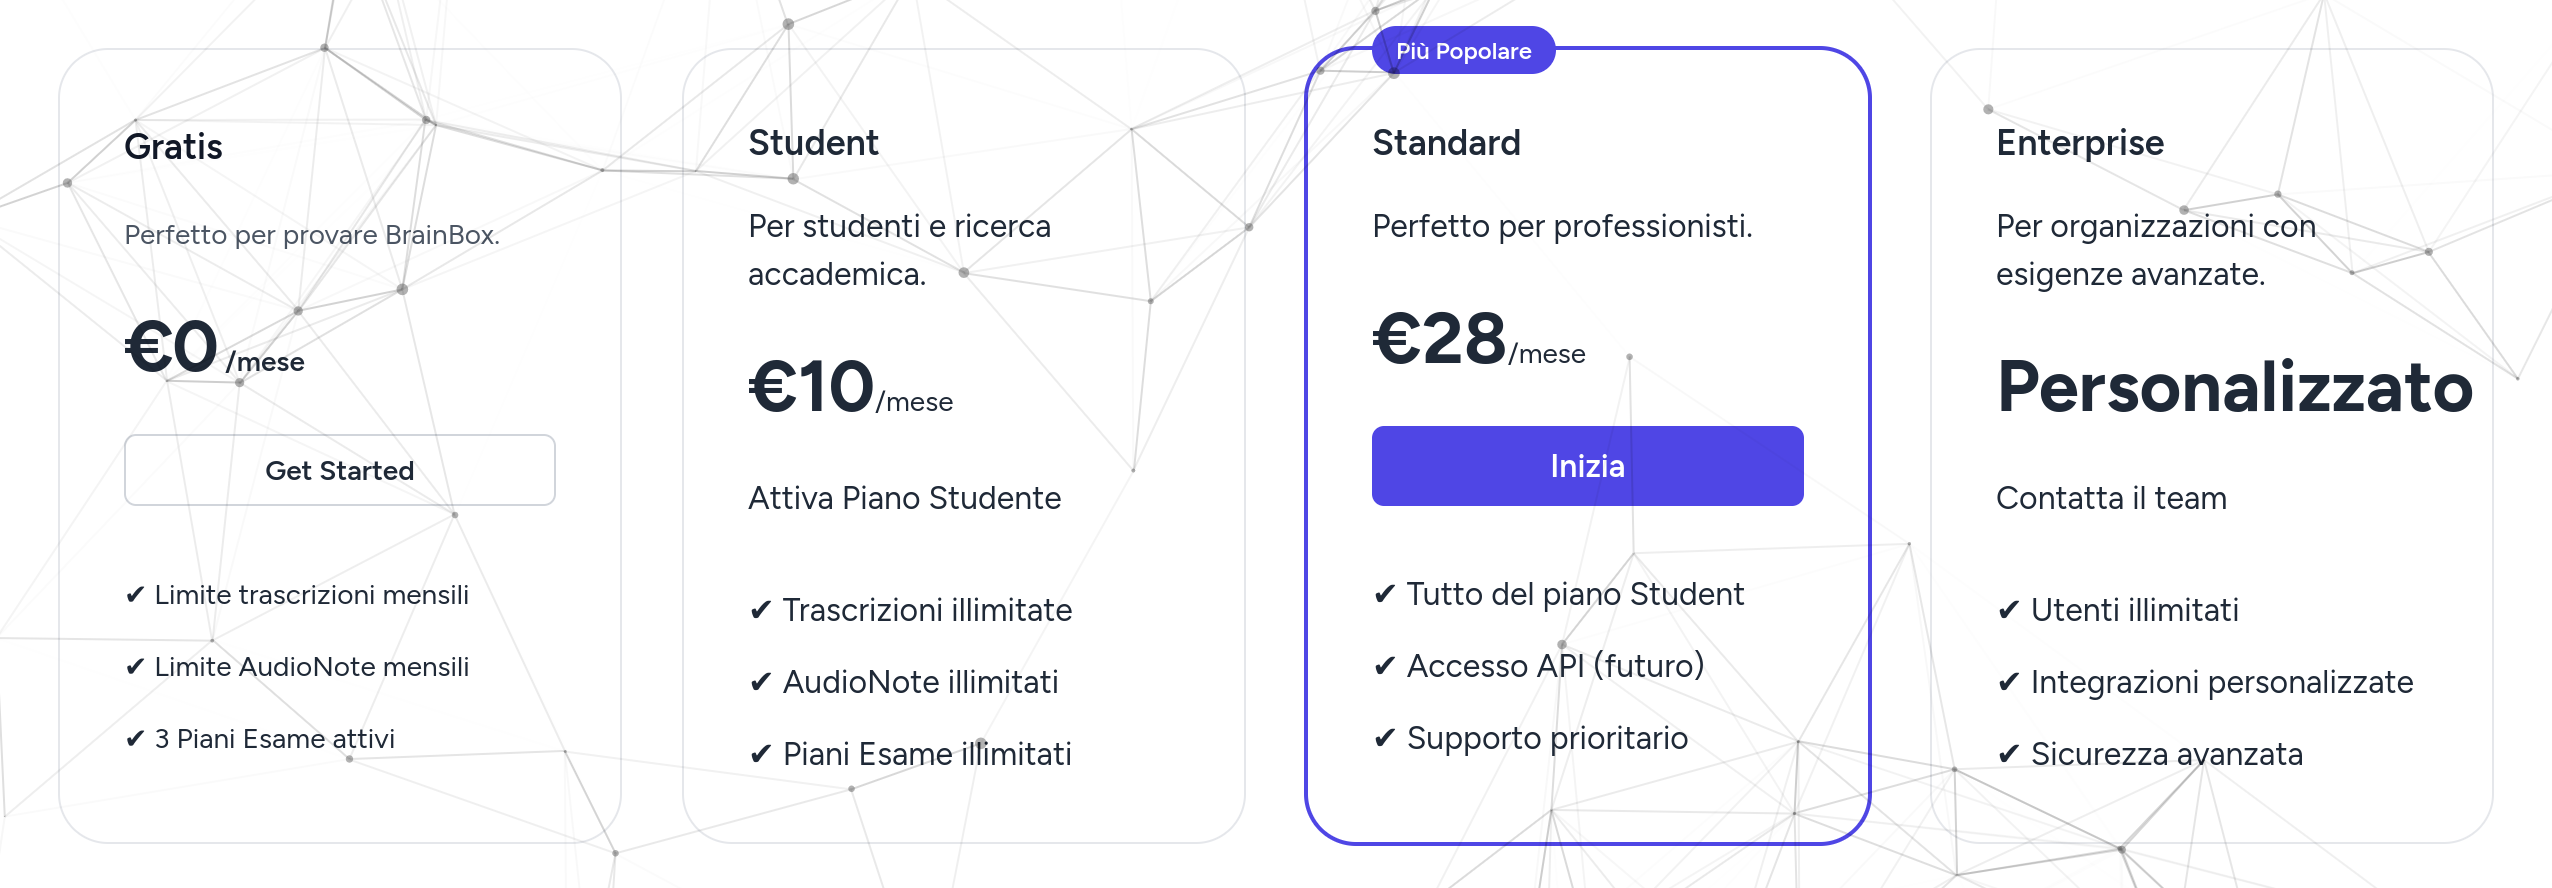
\includegraphics[width=6.5cm]{Screenshots/foglio1/Problema004.png}\hspace*{\fill}
    \vspace{10pt}
    \\
    \hline
    \textbf{Nome del valutatore} & Legati \\
    \hline
  \end{tabular}
\end{table}

% Problema \getNumeroProblema
\begin{table}[htbp]
  \centering
  \renewcommand{\arraystretch}{1.5}
  \begin{tabular}{|>{\raggedright\arraybackslash}p{7.5cm}|>{\raggedright\arraybackslash}p{7.5cm}|}
    \hline
    \rowcolor{green!30}
    \multicolumn{2}{|c|}{\textbf{Problema \getNumeroProblema}} \\
    \hline
    \textbf{Descrizione} & Nella sezione piani di abbonamento, il pulsante "Get Started" non è cliccabile. \\
    \hline
    \textbf{Pagina del sito} & Homepage \\
    \hline
    \textbf{Principi violati} & 1 (Far vedere lo stato del sistema); 5 (Riconoscimento piuttosto che uso della memoria dell’utente);  \\
    \hline
    \textbf{Grado di severità} & 3 (Problema rilevante) \\
    \hline
    \textbf{Screen} &
    \vspace{10pt}
    \hspace*{\fill}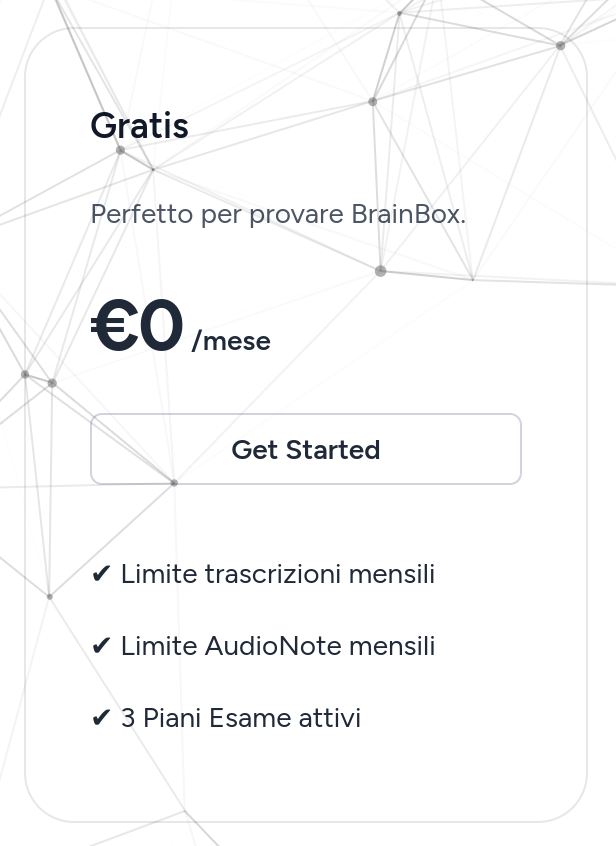
\includegraphics[width=6.5cm]{Screenshots/foglio1/Problema005.png}\hspace*{\fill}
    \vspace{10pt}
    \\
    \hline
    \textbf{Nome del valutatore} & Legati, Rinaldi, Kharef \\
    \hline
  \end{tabular}
\end{table}

% Problema \getNumeroProblema
\begin{table}[htbp]
  \centering
  \renewcommand{\arraystretch}{1.5}
  \begin{tabular}{|>{\raggedright\arraybackslash}p{7.5cm}|>{\raggedright\arraybackslash}p{7.5cm}|}
    \hline
    \rowcolor{green!30}
    \multicolumn{2}{|c|}{\textbf{Problema \getNumeroProblema}} \\
    \hline
    \textbf{Descrizione} & Il piano di abbonamento "Standard" ha un pulsante "Inizia" che non risulta cliccabile. \\
    \hline
    \textbf{Pagina del sito} & Homepage \\
    \hline
    \textbf{Principi violati} & 1 (Far vedere lo stato del sistema); 5 (Riconoscimento piuttosto che uso della memoria dell’utente);  \\
    \hline
    \textbf{Grado di severità} & 3 (Problema rilevante) \\
    \hline
    \textbf{Screen} &
    \vspace{10pt}
    \hspace*{\fill}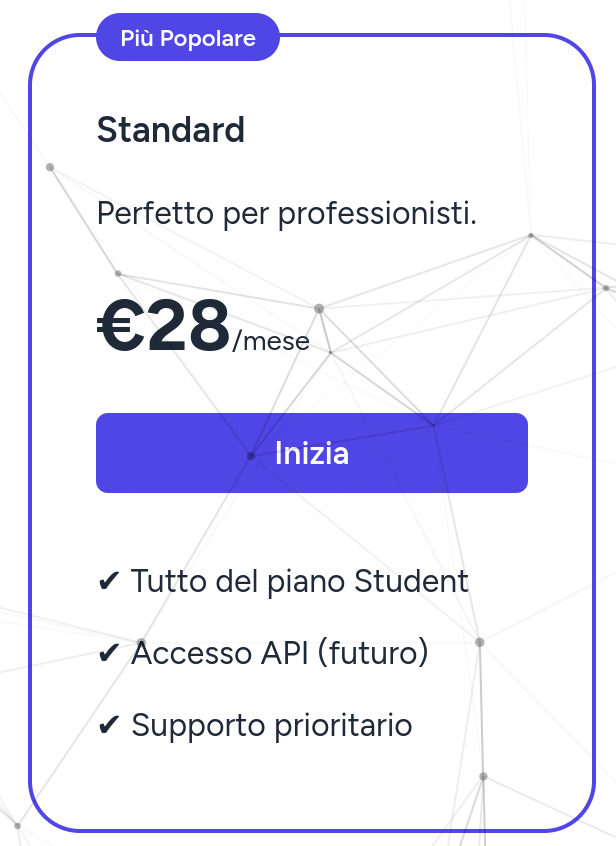
\includegraphics[width=6.5cm]{Screenshots/foglio1/Problema006.png}\hspace*{\fill}
    \vspace{10pt}
    \\
    \hline
    \textbf{Nome del valutatore} & Legati, Rinaldi, Kharef \\
    \hline
  \end{tabular}
\end{table}

% Problema \getNumeroProblema
\begin{table}[htbp]
  \centering
  \renewcommand{\arraystretch}{1.5}
  \begin{tabular}{|>{\raggedright\arraybackslash}p{7.5cm}|>{\raggedright\arraybackslash}p{7.5cm}|}
    \hline
    \rowcolor{green!30}
    \multicolumn{2}{|c|}{\textbf{Problema \getNumeroProblema}} \\
    \hline
    \textbf{Descrizione} & Il bottone in basso "Inizia Subito, Gratis" ha un testo diverso rispetto agli altri bottoni che hanno lo stesso comportamento. \\
    \hline
    \textbf{Pagina del sito} & Homepage \\
    \hline
    \textbf{Principi violati} & 4 (Assicurare consistenza); 5 (Riconoscimento piuttosto che uso della memoria dell'utente) \\
    \hline
    \textbf{Grado di severità} & 1 (Problema accessorio) \\
    \hline
    \textbf{Screen} &
    \vspace{10pt}
    \hspace*{\fill}
\includegraphics[width=6.5cm]{Screenshots/foglio1/Problema007.png}\hspace*{\fill}
    \vspace{10pt}
    \\
    \hline
    \textbf{Nome del valutatore} & Legati \\
    \hline
  \end{tabular}
\end{table}

% Problema \getNumeroProblema
\begin{table}[htbp]
  \centering
  \renewcommand{\arraystretch}{1.5}
  \begin{tabular}{|>{\raggedright\arraybackslash}p{7.5cm}|>{\raggedright\arraybackslash}p{7.5cm}|}
    \hline
    \rowcolor{green!30}
    \multicolumn{2}{|c|}{\textbf{Problema \getNumeroProblema}} \\
    \hline
    \textbf{Descrizione} & Nel footer della homepage, i link sotto le sezioni "Azienda" e "Legale" non funzionano. \\
    \hline
    \textbf{Pagina del sito} & Homepage \\
    \hline
    \textbf{Principi violati} & 1 (Far vedere lo stato del sistema); 5 (Riconoscimento piuttosto che uso della memoria dell’utente) \\
    \hline
    \textbf{Grado di severità} & 2 (Problema secondario) \\
    \hline
    \textbf{Screen} &
    \vspace{10pt}
    \hspace*{\fill}
\includegraphics[width=6.5cm]{Screenshots/foglio1/Problema008.png}\hspace*{\fill}
    \vspace{10pt}
    \\
    \hline
    \textbf{Nome del valutatore} & Legati, Rinaldi \\
    \hline
  \end{tabular}
\end{table}

% Problema \getNumeroProblema
\begin{table}[htbp]
  \centering
  \renewcommand{\arraystretch}{1.5}
  \begin{tabular}{|>{\raggedright\arraybackslash}p{7.5cm}|>{\raggedright\arraybackslash}p{7.5cm}|}
    \hline
    \rowcolor{green!30}
    \multicolumn{2}{|c|}{\textbf{Problema \getNumeroProblema}} \\
    \hline
    \textbf{Descrizione} & Il testo nei form di login e registrazione (inclusi i messaggi di errore) è in inglese, non coerente con la homepage in italiano. \\
    \hline
    \textbf{Pagina del sito} & Registrazione e Login \\
    \hline
    \textbf{Principi violati} & 2 (Adeguare il sistema al mondo reale); 4 (Assicurare consistenza); 9 (Permettere all’utente di correggere gli errori e non solo di rilevarli)  \\
    \hline
    \textbf{Grado di severità} & 2 (Problema secondario) \\
    \hline
    \textbf{Screen} &
    \vspace{10pt}
    \hspace*{\fill}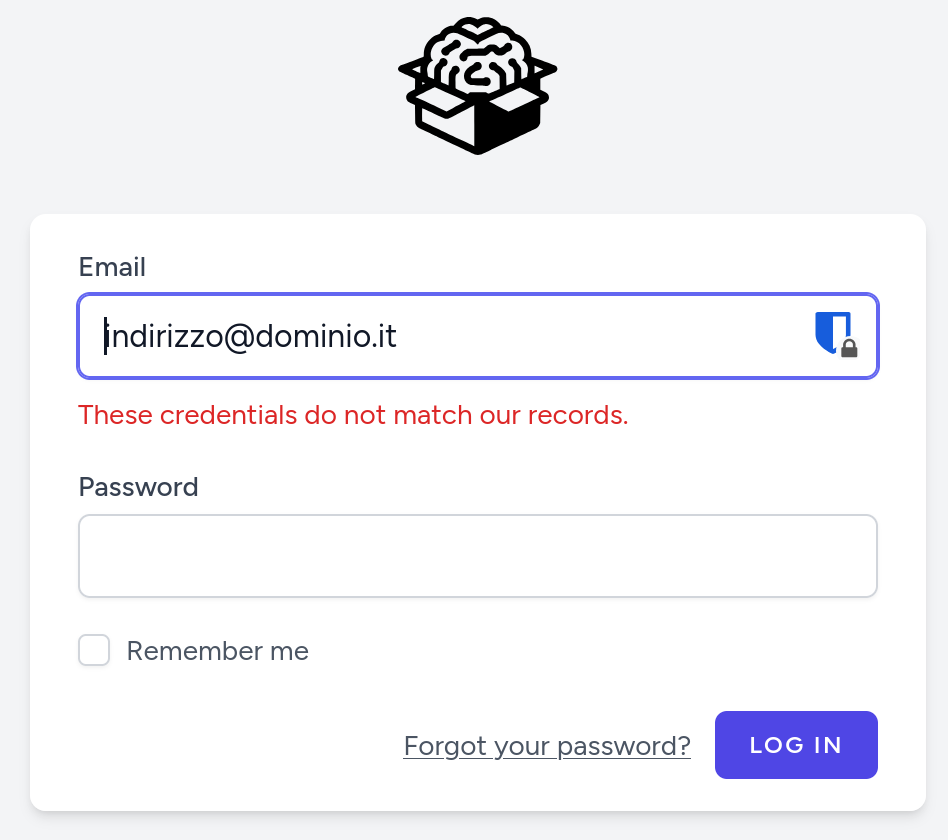
\includegraphics[width=6.5cm]{Screenshots/foglio1/Problema009.png}\hspace*{\fill}
    \vspace{10pt}
    \\
    \hline
    \textbf{Nome del valutatore} & Legati, Rinaldi, Kharef \\
    \hline
  \end{tabular}
\end{table}

% Problema \getNumeroProblema
\begin{table}[htbp]
  \centering
  \renewcommand{\arraystretch}{1.5}
  \begin{tabular}{|>{\raggedright\arraybackslash}p{7.5cm}|>{\raggedright\arraybackslash}p{7.5cm}|}
    \hline
    \rowcolor{green!30}
    \multicolumn{2}{|c|}{\textbf{Problema \getNumeroProblema}} \\
    \hline
    \textbf{Descrizione} & Dalle pagine di registrazione e di login non è possibile tornare alla homepage.\\
    \hline
    \textbf{Pagina del sito} & Registrazione e Login \\
    \hline
    \textbf{Principi violati} & 3 (Controllo dell'utente e libertà); 6 (Assicurare flessibilità ed efficienza d’uso) \\
    \hline
    \textbf{Grado di severità} & 2 (Problema secondario) \\
    \hline
    \textbf{Screen} &
    \vspace{10pt}
    \hspace*{\fill}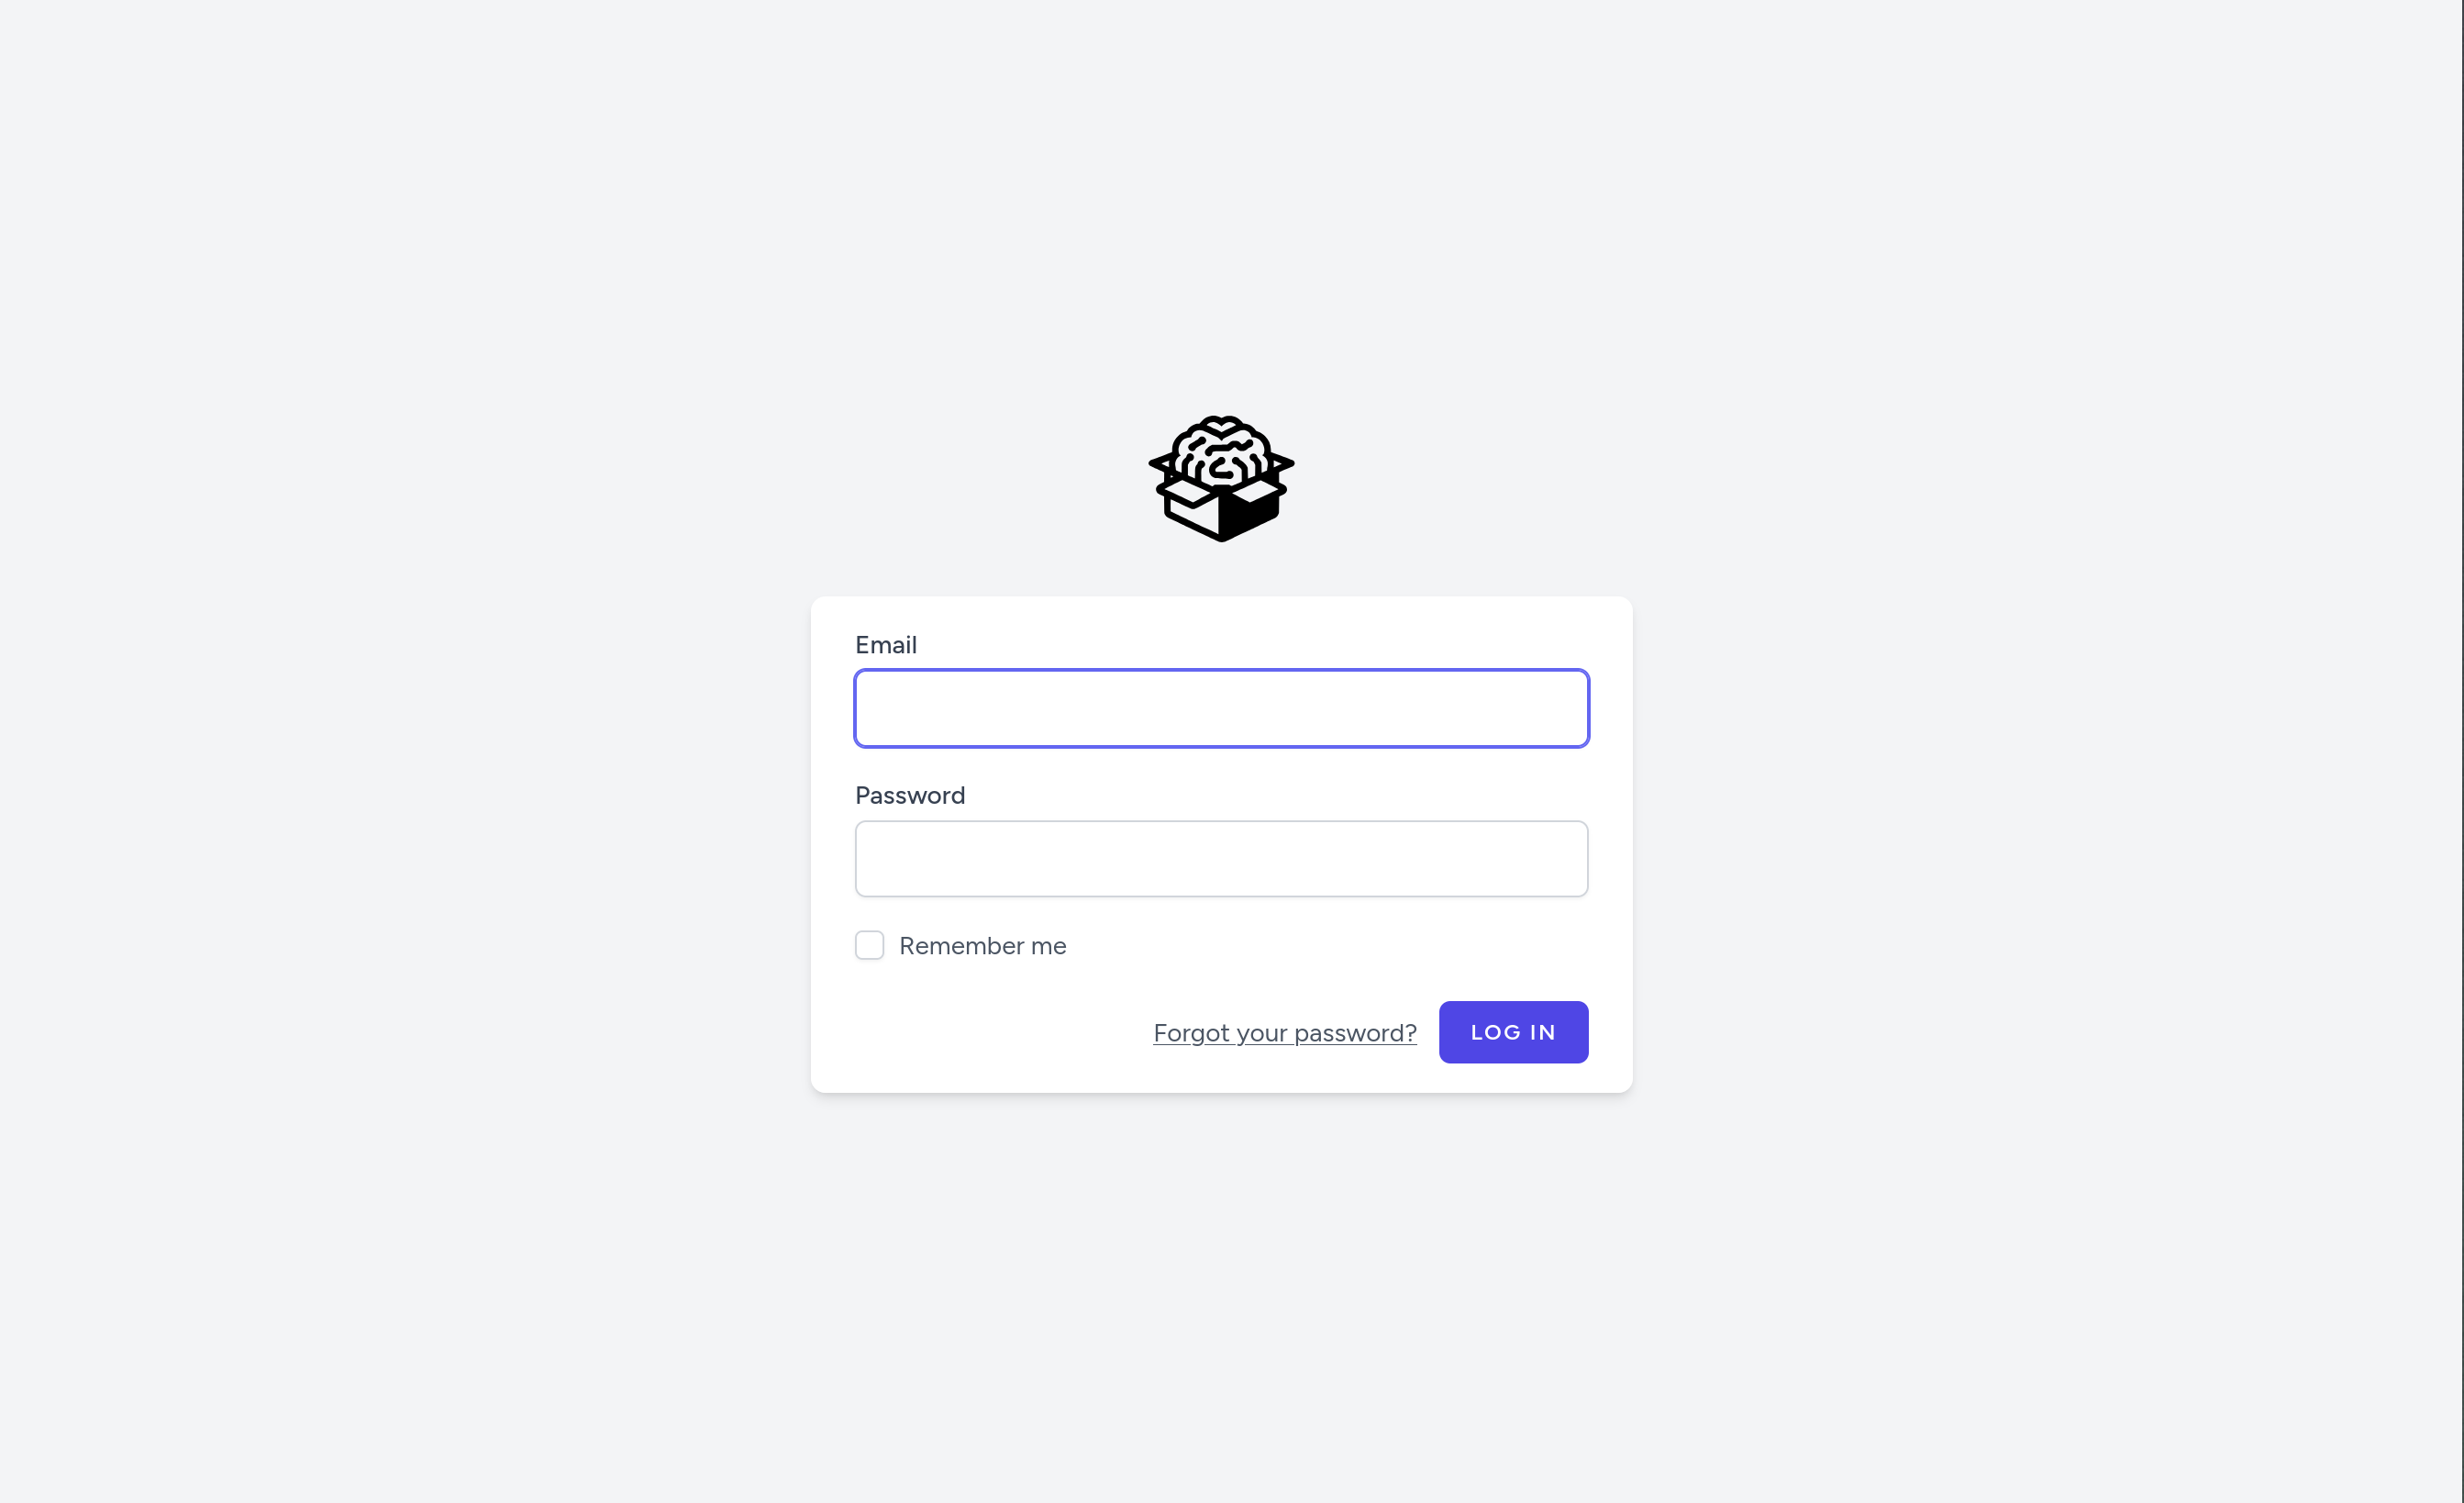
\includegraphics[width=6.5cm]{Screenshots/foglio1/Problema010.png}\hspace*{\fill}
    \vspace{10pt}
    \\
    \hline
    \textbf{Nome del valutatore} & Legati \\
    \hline
  \end{tabular}
\end{table}

% Problema \getNumeroProblema
\begin{table}[htbp]
  \centering
  \renewcommand{\arraystretch}{1.5}
  \begin{tabular}{|>{\raggedright\arraybackslash}p{7.5cm}|>{\raggedright\arraybackslash}p{7.5cm}|}
    \hline
    \rowcolor{green!30}
    \multicolumn{2}{|c|}{\textbf{Problema \getNumeroProblema}} \\
    \hline
    \textbf{Descrizione} & Nella dashboard, titoli, etichette e blocchi di testo sono un mix di italiano e inglese, compromettendo la coerenza linguistica. \\
    \hline
    \textbf{Pagina del sito} & Dashboard \\
    \hline
    \textbf{Principi violati} & 2 (Adeguare il sistema al mondo reale); 4 (Assicurare consistenza) \\
    \hline
    \textbf{Grado di severità} & 2 (Problema secondario) \\
    \hline
    \textbf{Screen} &
    \vspace{10pt}
    \hspace*{\fill}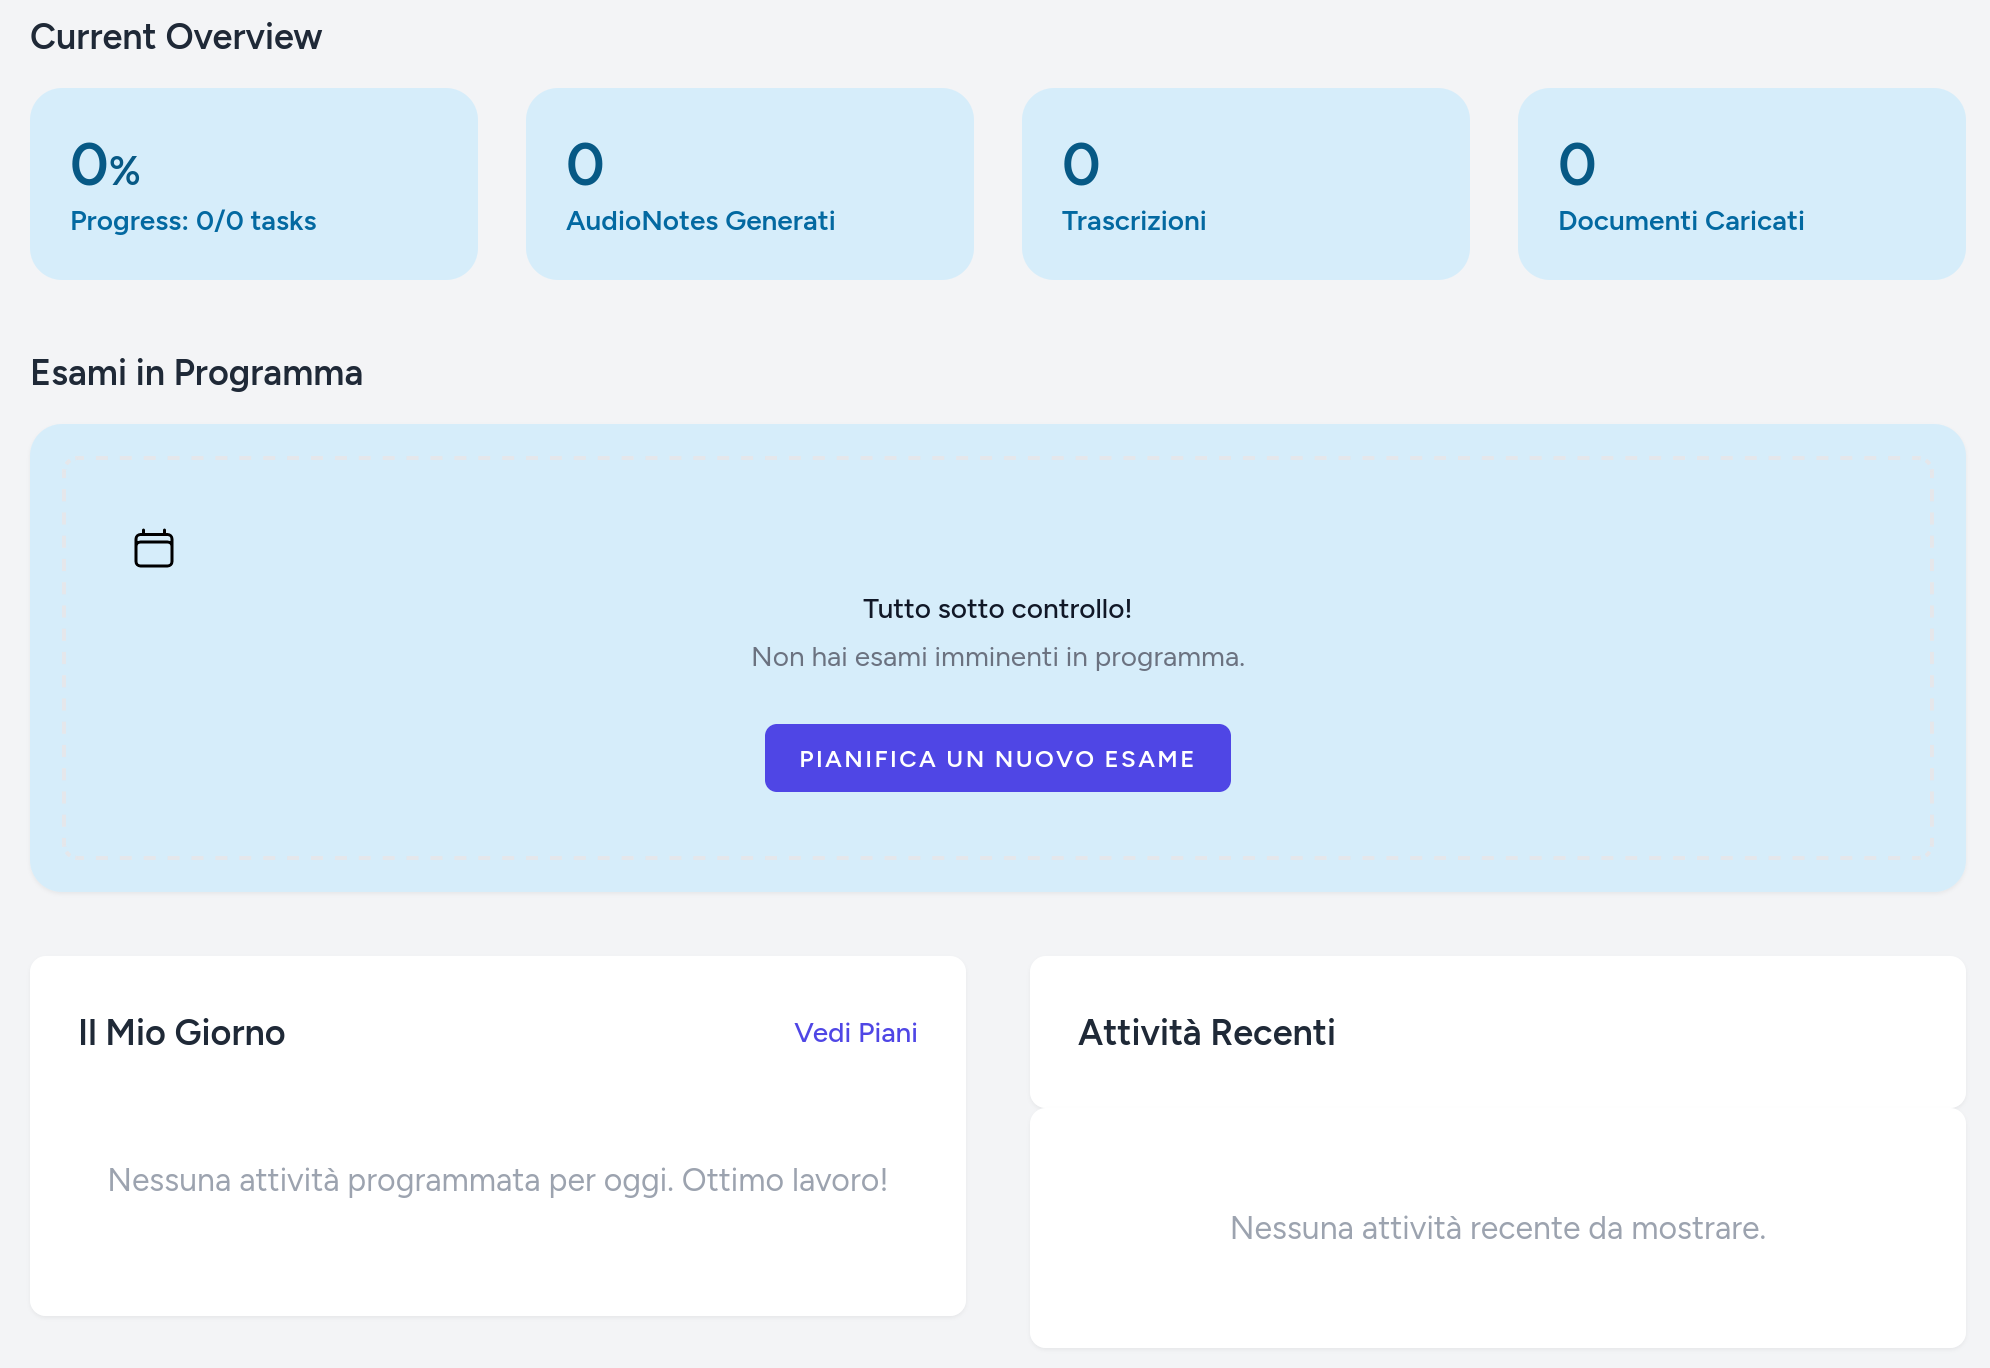
\includegraphics[width=6.5cm]{Screenshots/foglio1/Problema011.png}\hspace*{\fill}
    \vspace{10pt}
    \\
    \hline
    \textbf{Nome del valutatore} & Legati, Rinaldi, Kharef \\
    \hline
  \end{tabular}
\end{table}

% Problema \getNumeroProblema
\begin{table}[htbp]
  \centering
  \renewcommand{\arraystretch}{1.5}
  \begin{tabular}{|>{\raggedright\arraybackslash}p{7.5cm}|>{\raggedright\arraybackslash}p{7.5cm}|}
    \hline
    \rowcolor{green!30}
    \multicolumn{2}{|c|}{\textbf{Problema \getNumeroProblema}} \\
    \hline
    \textbf{Descrizione} & Il pulsante in alto a destra per le notifiche non è funzionante. \\
    \hline
    \textbf{Pagina del sito} & Dashboard \\
    \hline
    \textbf{Principi violati} & 1 (Far vedere lo stato del sistema); \\
    \hline
    \textbf{Grado di severità} & 4 (Catastrofe di usabilità) \\
    \hline
    \textbf{Screen} &
    \vspace{10pt}
    \hspace*{\fill}
\includegraphics[width=6.5cm]{Screenshots/foglio1/Problema012.png}\hspace*{\fill}
    \vspace{10pt}
    \\
    \hline
    \textbf{Nome del valutatore} & Legati, Rinaldi, Kharef \\
    \hline
  \end{tabular}
\end{table}

% Problema \getNumeroProblema
\begin{table}[htbp]
  \centering
  \renewcommand{\arraystretch}{1.5}
  \begin{tabular}{|>{\raggedright\arraybackslash}p{7.5cm}|>{\raggedright\arraybackslash}p{7.5cm}|}
    \hline
    \rowcolor{green!30}
    \multicolumn{2}{|c|}{\textbf{Problema \getNumeroProblema}} \\
    \hline
    \textbf{Descrizione} & Nelle impostazioni del profilo, il testo è scritto interamente in inglese. \\
    \hline
    \textbf{Pagina del sito} & Dashboard - Profilo \\
    \hline
    \textbf{Principi violati} & 2 (Adeguare il sistema al mondo reale) \\
    \hline
    \textbf{Grado di severità} & 2 (Problema secondario) \\
    \hline
    \textbf{Screen} &
    \vspace{10pt}
    \hspace*{\fill}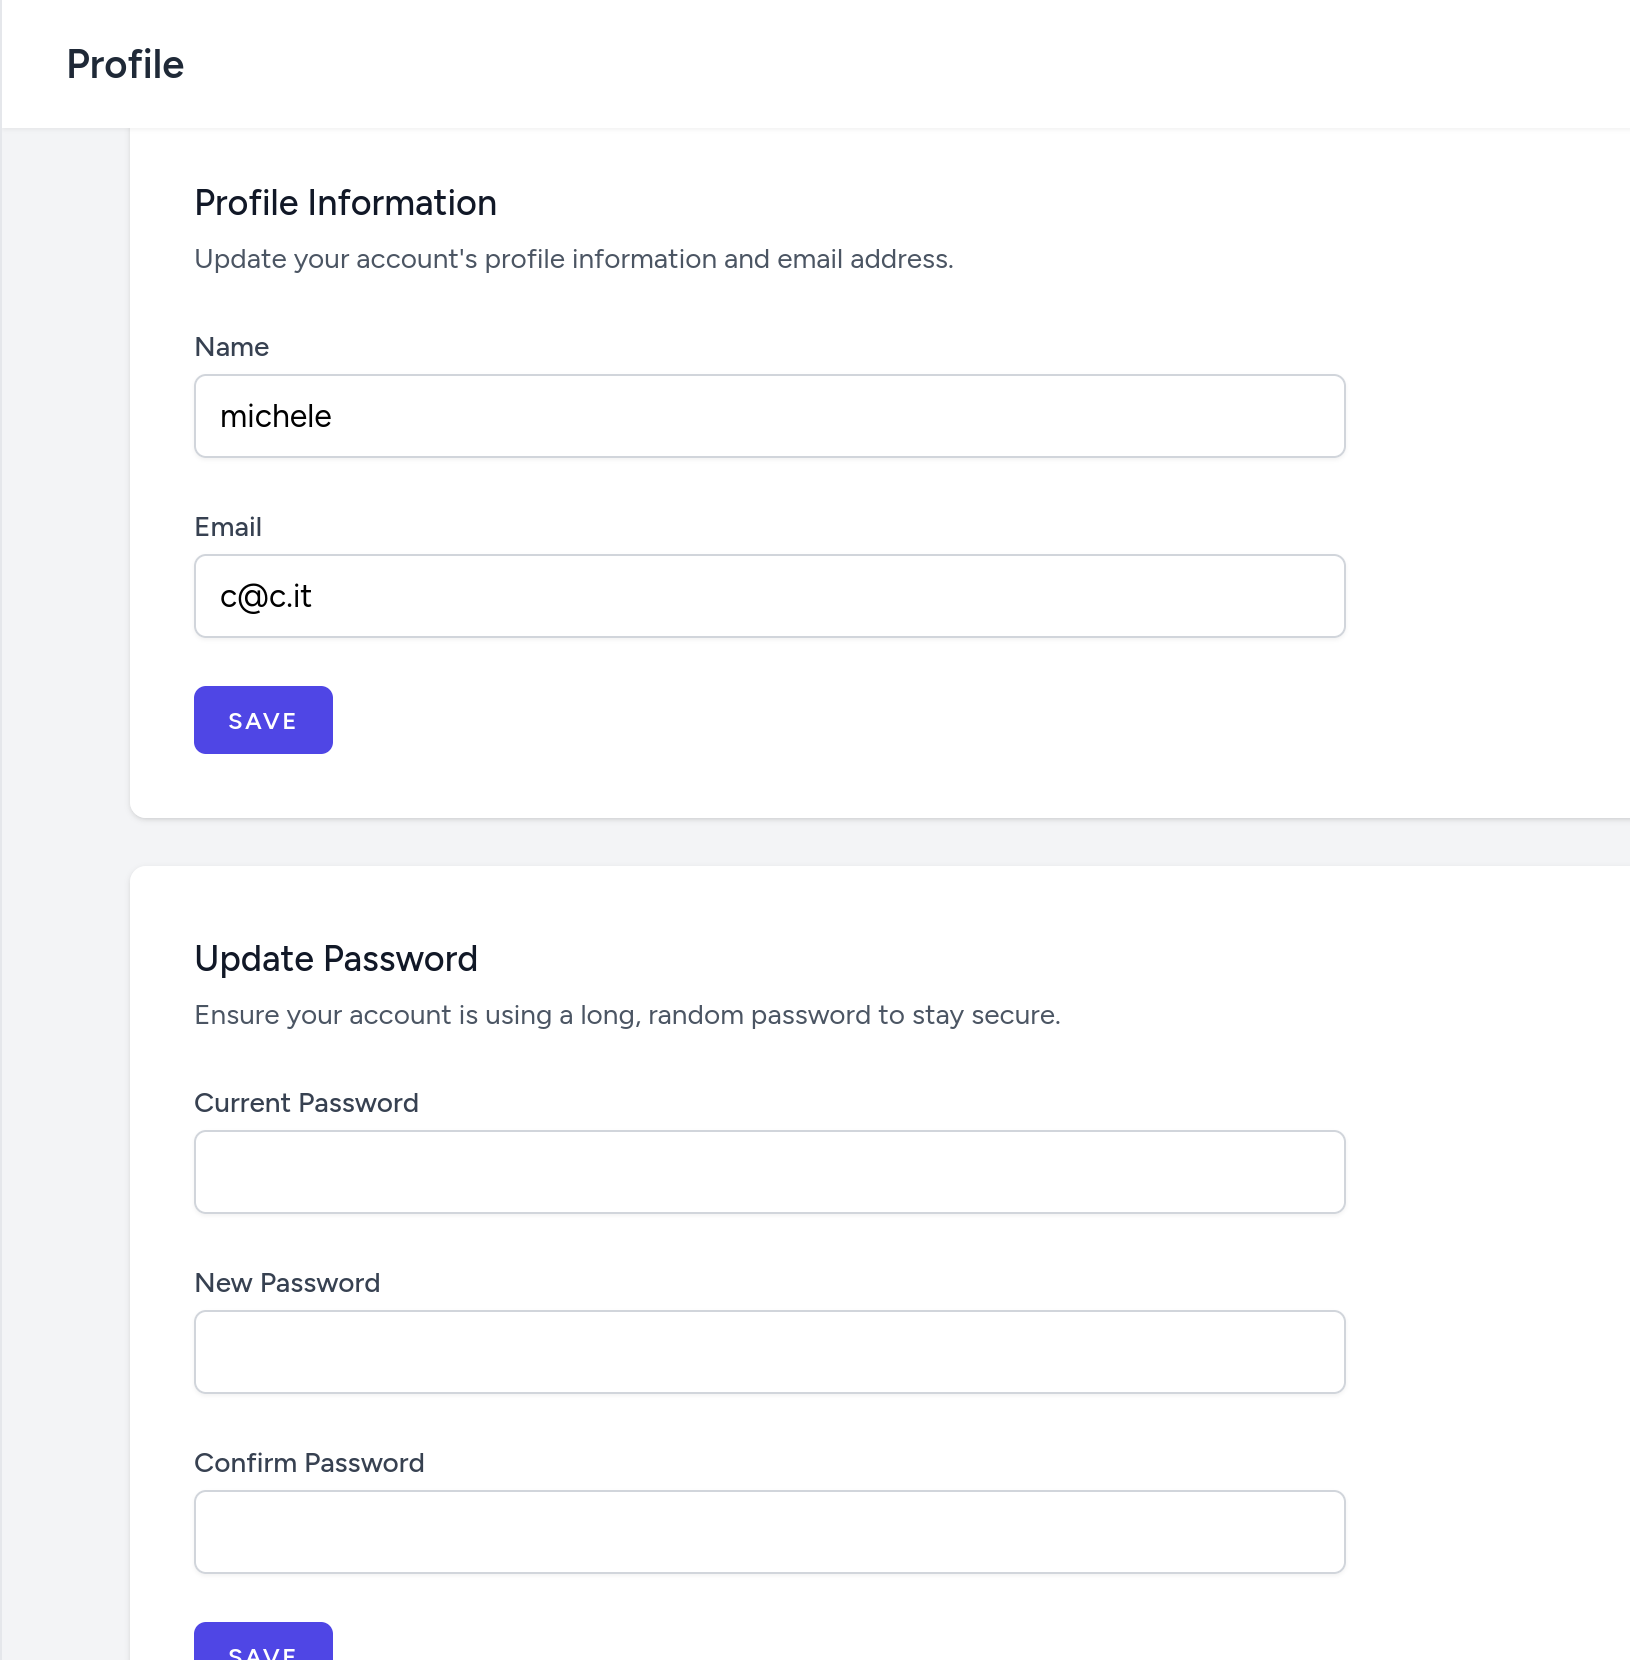
\includegraphics[width=6.5cm]{Screenshots/foglio1/Problema013.png}\hspace*{\fill}
    \vspace{10pt}
    \\
    \hline
    \textbf{Nome del valutatore} & Legati, Rinaldi \\
    \hline
  \end{tabular}
\end{table}

% Problema \getNumeroProblema
\begin{table}[htbp]
  \centering
  \renewcommand{\arraystretch}{1.5}
  \begin{tabular}{|>{\raggedright\arraybackslash}p{7.5cm}|>{\raggedright\arraybackslash}p{7.5cm}|}
    \hline
    \rowcolor{green!30}
    \multicolumn{2}{|c|}{\textbf{Problema \getNumeroProblema}} \\
    \hline
    \textbf{Descrizione} & Il pulsante di logout non chiede conferma all'utente prima di disconnettersi. \\
    \hline
    \textbf{Pagina del sito} & Dashboard - Logout \\
    \hline
    \textbf{Principi violati} & 8 (Prevenire gli errori); 9 (Permettere all'utente di correggere gli errori) \\
    \hline
    \textbf{Grado di severità} & 2 (Problema secondario) \\
    \hline
    \textbf{Screen} &
    \vspace{10pt}
    \hspace*{\fill}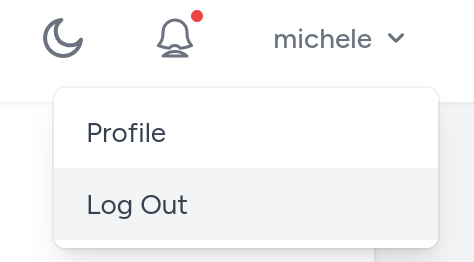
\includegraphics[width=6.5cm]{Screenshots/foglio1/Problema014.png}\hspace*{\fill}
    \vspace{10pt}
    \\
    \hline
    \textbf{Nome del valutatore} & Legati, Rinaldi \\
    \hline
  \end{tabular}
\end{table}

% Problema \getNumeroProblema
\begin{table}[htbp]
  \centering
  \renewcommand{\arraystretch}{1.5}
  \begin{tabular}{|>{\raggedright\arraybackslash}p{7.5cm}|>{\raggedright\arraybackslash}p{7.5cm}|}
    \hline
    \rowcolor{green!30}
    \multicolumn{2}{|c|}{\textbf{Problema \getNumeroProblema}} \\
    \hline
    \textbf{Descrizione} & La modalità notte rende alcuni testi poco visibili, compromettendo la leggibilità. \\
    \hline
    \textbf{Pagina del sito} & Dashboard \\
    \hline
    \textbf{Principi violati} & 5 (Riconoscimento piuttosto che uso della memoria dell’utente); 7 (Visualizzare tutte e sole le informazioni necessarie) \\
    \hline
    \textbf{Grado di severità} & 2 (Problema secondario) \\
    \hline
    \textbf{Screen} &
    \vspace{10pt}
    \hspace*{\fill}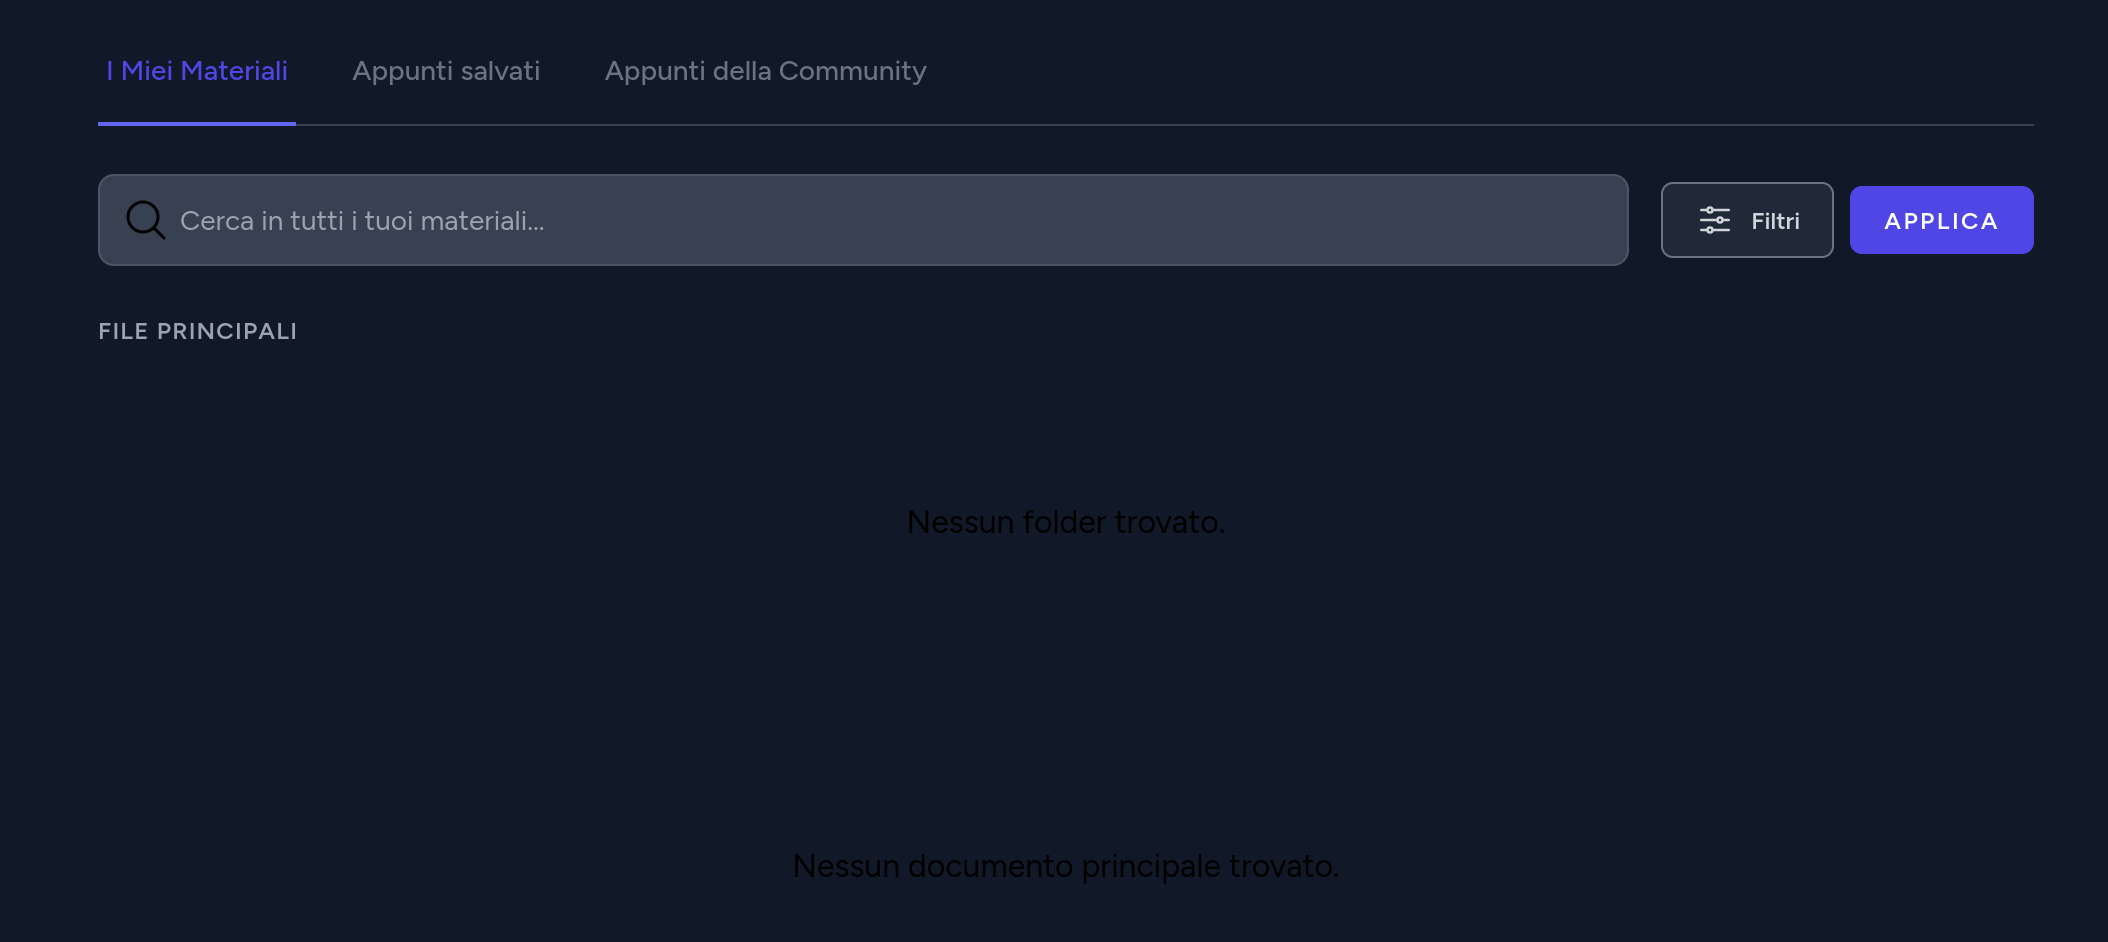
\includegraphics[width=6.5cm]{Screenshots/foglio1/Problema015.png}\hspace*{\fill}
    \vspace{10pt}
    \\
    \hline
    \textbf{Nome del valutatore} & Legati, Kharef \\
    \hline
  \end{tabular}
\end{table}

% Problema \getNumeroProblema
\begin{table}[htbp]
  \centering
  \renewcommand{\arraystretch}{1.5}
  \begin{tabular}{|>{\raggedright\arraybackslash}p{7.5cm}|>{\raggedright\arraybackslash}p{7.5cm}|}
    \hline
    \rowcolor{green!30}
    \multicolumn{2}{|c|}{\textbf{Problema \getNumeroProblema}} \\
    \hline
    \textbf{Descrizione} & In modalità notte, la selezione di qualsiasi pulsante con una funzione genera un effetto "flash" (l'interfaccia torna brevemente alla modalità chiara). \\
    \hline
    \textbf{Pagina del sito} & Dashboard \\
    \hline
    \textbf{Principi violati} & 4 (Assicurare consistenza) \\
    \hline
    \textbf{Grado di severità} & 3 (Problema rilevante) \\ \\
    \hline
    \textbf{Nome del valutatore} & Rinaldi \\
    \hline
  \end{tabular}
\end{table}

% Problema \getNumeroProblema
\begin{table}[htbp]
  \centering
  \renewcommand{\arraystretch}{1.5}
  \begin{tabular}{|>{\raggedright\arraybackslash}p{7.5cm}|>{\raggedright\arraybackslash}p{7.5cm}|}
    \hline
    \rowcolor{green!30}
    \multicolumn{2}{|c|}{\textbf{Problema \getNumeroProblema}} \\
    \hline
    \textbf{Descrizione} & Il pulsante in basso a destra "Passa a BrainBox Pro +" non è funzionante e non rimanda a nulla. \\
    \hline
    \textbf{Pagina del sito} & Dashboard \\
    \hline
    \textbf{Principi violati} & 1 (Far vedere lo stato del sistema); 5 (Riconoscimento piuttosto che uso della memoria dell’utente) \\
    \hline
    \textbf{Grado di severità} & 3 (Problema rilevante) \\
    \hline
    \textbf{Screen} &
    \vspace{10pt}
    \hspace*{\fill}
\includegraphics[width=6.5cm]{Screenshots/foglio1/Problema017.png}\hspace*{\fill}
    \vspace{10pt}
    \\
    \hline
    \textbf{Nome del valutatore} & Legati, Rinaldi, Kharef \\
    \hline
  \end{tabular}
\end{table}

% Problema \getNumeroProblema
\begin{table}[htbp]
  \centering
  \renewcommand{\arraystretch}{1.5}
  \begin{tabular}{|>{\raggedright\arraybackslash}p{7.5cm}|>{\raggedright\arraybackslash}p{7.5cm}|}
    \hline
    \rowcolor{green!30}
    \multicolumn{2}{|c|}{\textbf{Problema \getNumeroProblema}} \\
    \hline
    \textbf{Descrizione} & Nei campi password dei form di login e registrazione non è possibile visualizzare la password inserita. \\
    \hline
    \textbf{Pagina del sito} & Registrazione e Login \\
    \hline
    \textbf{Principi violati} & 1 (Far vedere lo stato del sistema); 5 (Riconoscimento piuttosto che uso della memoria dell'utente); 6 (Assicurare flessibilità ed efficienza d'uso) \\
    \hline
    \textbf{Grado di severità} & 3 (Problema rilevante) \\
    \hline
    \textbf{Screen} &
    \vspace{10pt}
    \hspace*{\fill}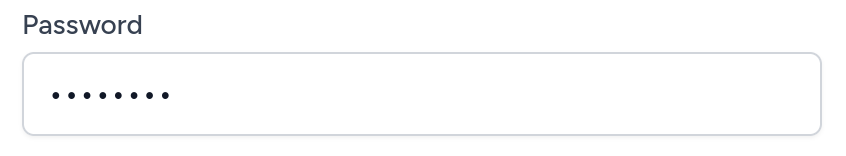
\includegraphics[width=6.5cm]{Screenshots/foglio1/Problema018.png}\hspace*{\fill}
    \vspace{10pt}
    \\
    \hline
    \textbf{Nome del valutatore} & Rinaldi \\
    \hline
  \end{tabular}
\end{table}

% Problema \getNumeroProblema
\begin{table}[htbp]
  \centering
  \renewcommand{\arraystretch}{1.5}
  \begin{tabular}{|>{\raggedright\arraybackslash}p{7.5cm}|>{\raggedright\arraybackslash}p{7.5cm}|}
    \hline
    \rowcolor{green!30}
    \multicolumn{2}{|c|}{\textbf{Problema \getNumeroProblema}} \\
    \hline
    \textbf{Descrizione} & Nella sezione "Completa il tuo profilo" (della registrazione) il menu a tendina consente di selezionare la voce "Seleziona la tua università" (che non dovrebbe essere selezionabile), analogamente a quanto avviene per i campi "Dipartimento" e "Ciclo di studi". \\
    \hline
    \textbf{Pagina del sito} & Registrazione \\
    \hline
    \textbf{Principi violati} & 7 (Visualizzare tutte e sole le informazioni necessarie); 8 (Prevenire gli errori) \\
    \hline
    \textbf{Grado di severità} & 2 (Problema secondario) \\
    \hline
    \textbf{Screen} &
    \vspace{10pt}
    \hspace*{\fill}
\includegraphics[width=6.5cm]{Screenshots/foglio1/Problema019.png}\hspace*{\fill}
    \vspace{10pt}
    \\
    \hline
    \textbf{Nome del valutatore} & Rinaldi \\
    \hline
  \end{tabular}
\end{table}

% Problema \getNumeroProblema (Basato su Legati [2])
\begin{table}[htbp]
  \centering
  \renewcommand{\arraystretch}{1.5}
  \begin{tabular}{|>{\raggedright\arraybackslash}p{7.5cm}|>{\raggedright\arraybackslash}p{7.5cm}|}
    \hline
    \rowcolor{green!30}
    \multicolumn{2}{|c|}{\textbf{Problema \getNumeroProblema}} \\
    \hline
    \textbf{Descrizione} & Nella pagina "I Miei Appunti", il titolo della pagina è scritto in inglese. \\
    \hline
    \textbf{Pagina del sito} & Dashboard - I Miei Appunti \\
    \hline
    \textbf{Principi violati} & 2 (Adeguare il sistema al mondo reale); 4 (Assicurare consistenza) \\
    \hline
    \textbf{Grado di severità} & 2 (Problema secondario) \\
    \hline
    \textbf{Screen} &
    \vspace{10pt}
    \hspace*{\fill}
\includegraphics[width=6.5cm]{Screenshots/foglio1/Problema021.png}\hspace*{\fill}
    \vspace{10pt}
    \\
    \hline
    \textbf{Nome del valutatore} & Legati, Rinaldi, Kharef \\
    \hline
  \end{tabular}
\end{table}

% Problema \getNumeroProblema (Basato su Legati [2])
\begin{table}[htbp]
  \centering
  \renewcommand{\arraystretch}{1.5}
  \begin{tabular}{|>{\raggedright\arraybackslash}p{7.5cm}|>{\raggedright\arraybackslash}p{7.5cm}|}
    \hline
    \rowcolor{green!30}
    \multicolumn{2}{|c|}{\textbf{Problema \getNumeroProblema}} \\
    \hline
    \textbf{Descrizione} & Nella pagina "I Miei Appunti", i pulsanti "CARICA FILE" e "Nuova Cartella" sono posizionati in un punto poco coerente con il contenuto della pagina. \\
    \hline
    \textbf{Pagina del sito} & Dashboard - I Miei Appunti \\
    \hline
    \textbf{Principi violati} & 5 (Riconoscimento piuttosto che uso della memoria dell’utente) \\
    \hline
    \textbf{Grado di severità} & 1 (Problema accessorio) \\
    \hline
    \textbf{Screen} &
    \vspace{10pt}
    \hspace*{\fill}
\includegraphics[width=6.5cm]{Screenshots/foglio1/Problema022.png}\hspace*{\fill}
    \vspace{10pt}
    \\
    \hline
    \textbf{Nome del valutatore} & Legati \\
    \hline
  \end{tabular}
\end{table}

% Problema \getNumeroProblema (Basato su Legati [2])
\begin{table}[htbp]
  \centering
  \renewcommand{\arraystretch}{1.5}
  \begin{tabular}{|>{\raggedright\arraybackslash}p{7.5cm}|>{\raggedright\arraybackslash}p{7.5cm}|}
    \hline
    \rowcolor{green!30}
    \multicolumn{2}{|c|}{\textbf{Problema \getNumeroProblema}} \\
    \hline
    \textbf{Descrizione} & Nella pagina "I Miei Appunti", il pulsante "CARICA FILE" è scritto in maiuscolo a differenza di tutti gli altri pulsanti. \\
    \hline
    \textbf{Pagina del sito} & Dashboard - I Miei Appunti \\
    \hline
    \textbf{Principi violati} & 4 (Assicurare consistenza) \\
    \hline
    \textbf{Grado di severità} & 1 (Problema accessorio) \\
    \hline
    \textbf{Screen} &
    \vspace{10pt}
    \hspace*{\fill}
\includegraphics[width=6.5cm]{Screenshots/foglio1/Problema023.png}\hspace*{\fill}
    \vspace{10pt}
    \\
    \hline
    \textbf{Nome del valutatore} & Legati \\
    \hline
  \end{tabular}
\end{table}

% Problema \getNumeroProblema (Basato su Legati [2])
\begin{table}[htbp]
  \centering
  \renewcommand{\arraystretch}{1.5}
  \begin{tabular}{|>{\raggedright\arraybackslash}p{7.5cm}|>{\raggedright\arraybackslash}p{7.5cm}|}
    \hline
    \rowcolor{green!30}
    \multicolumn{2}{|c|}{\textbf{Problema \getNumeroProblema}} \\
    \hline
    \textbf{Descrizione} & Nella pagina "I Miei Appunti", il pulsante "CARICA FILE" ha un'icona che non rispecchia il comportamento del pulsante. \\
    \hline
    \textbf{Pagina del sito} & Dashboard - I Miei Appunti \\
    \hline
    \textbf{Principi violati} & 2 (Adeguare il sistema al mondo reale); 5 (Riconoscimento piuttosto che uso della memoria dell’utente) \\
    \hline
    \textbf{Grado di severità} & 2 (Problema secondario) \\
    \hline
    \textbf{Screen} &
    \vspace{10pt}
    \hspace*{\fill}
\includegraphics[width=6.5cm]{Screenshots/foglio1/Problema024.png}\hspace*{\fill}
    \vspace{10pt}
    \\
    \hline
    \textbf{Nome del valutatore} & Legati \\
    \hline
  \end{tabular}
\end{table}

% Problema \getNumeroProblema (Basato su Legati [4])
\begin{table}[htbp]
  \centering
  \renewcommand{\arraystretch}{1.5}
  \begin{tabular}{|>{\raggedright\arraybackslash}p{7.5cm}|>{\raggedright\arraybackslash}p{7.5cm}|}
    \hline
    \rowcolor{green!30}
    \multicolumn{2}{|c|}{\textbf{Problema \getNumeroProblema}} \\
    \hline
    \textbf{Descrizione} & Nella pagina "I Miei Appunti", il tab "I Miei Materiali" ha un titolo poco fuorviante per la pagina; dovrebbe essere "I Miei Appunti". \\
    \hline
    \textbf{Pagina del sito} & Dashboard - I Miei Appunti \\
    \hline
    \textbf{Principi violati} & 2 (Adeguare il sistema al mondo reale); 5 (Riconoscimento piuttosto che uso della memoria dell’utente) \\
    \hline
    \textbf{Grado di severità} & 1 (Problema accessorio) \\
    \hline
    \textbf{Screen} &
    \vspace{10pt}
    \hspace*{\fill}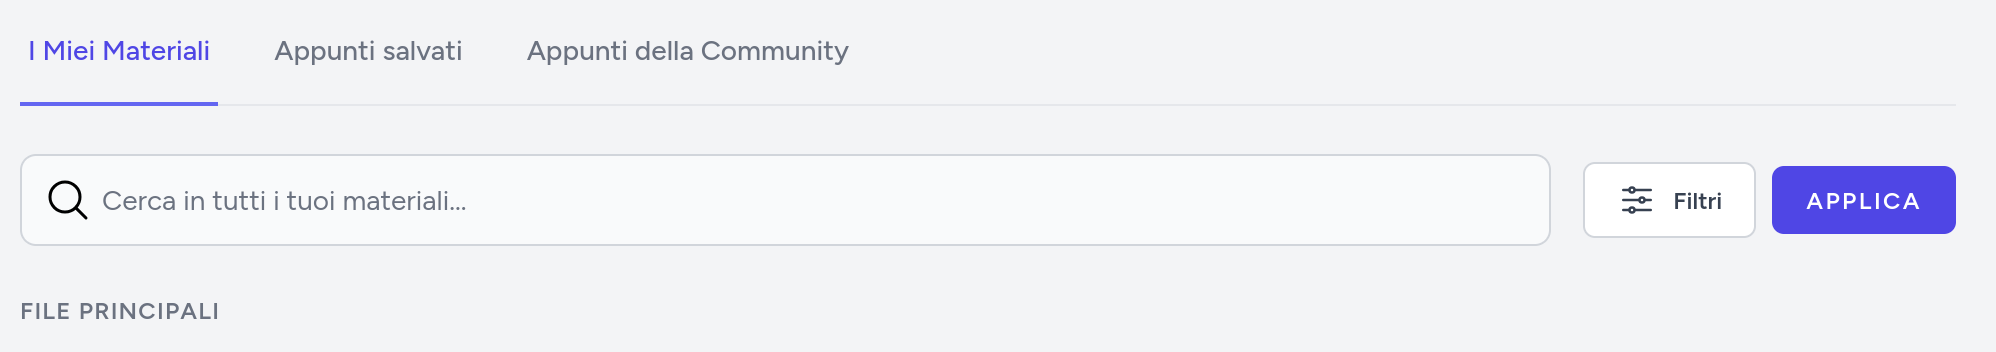
\includegraphics[width=6.5cm]{Screenshots/foglio1/Problema025.png}\hspace*{\fill}
    \vspace{10pt}
    \\
    \hline
    \textbf{Nome del valutatore} & Legati \\
    \hline
  \end{tabular}
\end{table}

% Problema \getNumeroProblema (Basato su Legati [4])
\begin{table}[htbp]
  \centering
  \renewcommand{\arraystretch}{1.5}
  \begin{tabular}{|>{\raggedright\arraybackslash}p{7.5cm}|>{\raggedright\arraybackslash}p{7.5cm}|}
    \hline
    \rowcolor{green!30}
    \multicolumn{2}{|c|}{\textbf{Problema \getNumeroProblema}} \\
    \hline
    \textbf{Descrizione} & Nella pagina "I Miei Appunti", una volta cliccato sul tab "Appunti Salvati" o "Appunti della Community", non è più possibile tornare indietro. Manca un pulsante o un percorso di navigazione che consenta di tornare alla pagina precedente. \\
    \hline
    \textbf{Pagina del sito} & Dashboard - I Miei Appunti \\
    \hline
    \textbf{Principi violati} & 3 (Controllo dell'utente e libertà); 6 (Assicurare flessibilità ed efficienza d’uso) \\
    \hline
    \textbf{Grado di severità} & 2 (Problema secondario) \\
    \hline
    \textbf{Screen} &
    \vspace{10pt}
    \hspace*{\fill}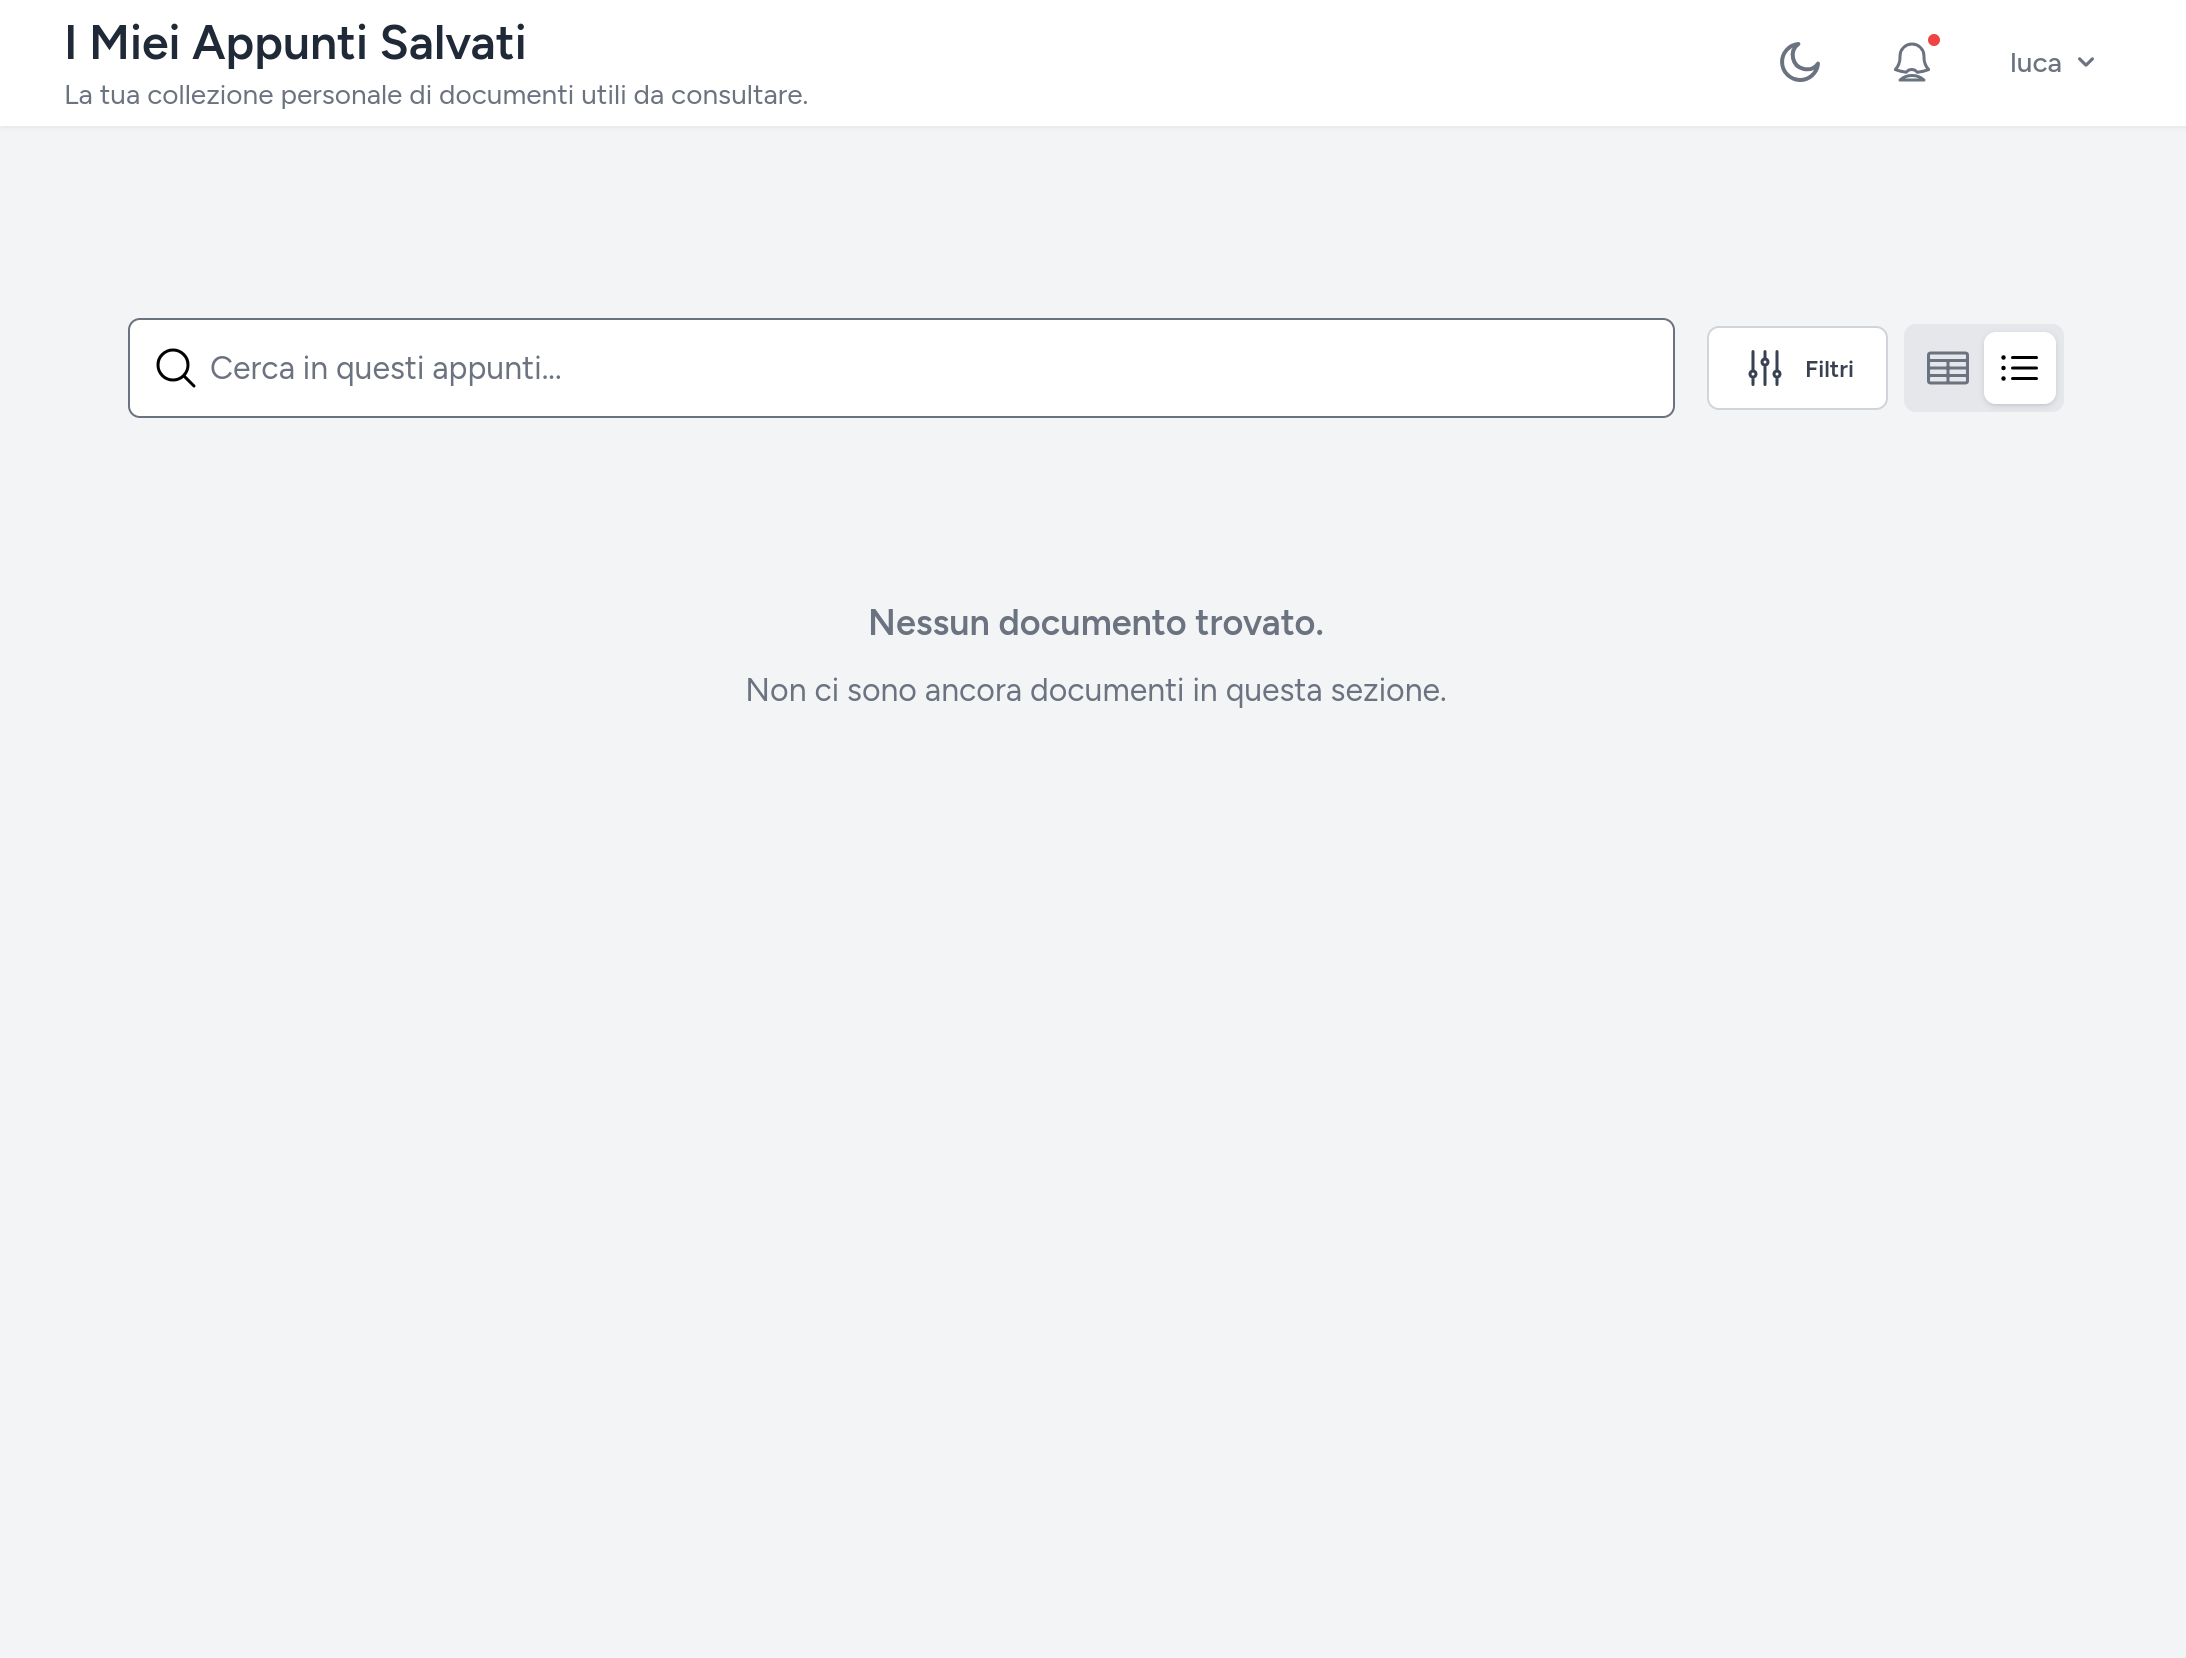
\includegraphics[width=6.5cm]{Screenshots/foglio1/Problema026.png}\hspace*{\fill}
    \vspace{10pt}
    \\
    \hline
    \textbf{Nome del valutatore} & Legati, Rinaldi \\
    \hline
  \end{tabular}
\end{table}